\documentclass{article}

% used for margins
\usepackage[letterpaper,left=1.25in,right=1.25in,top=1in,bottom=1in]{geometry}
% used for graphics
\usepackage{graphicx}
% used for eps graphics
\usepackage{epstopdf}

\pagestyle{plain}
\author{Kevin Nash}
\title{AirVille Design Document}

\begin{document}
\maketitle

\section{Introduction}

\subsection{Purpose}
This software design document describes the system architecture and design of
the gameplay portion of $AirVille$, a $Zonga$ game.

\subsection{Scope}
This document outlines the implementation details of $AirVille$. The software
will consist of the gameplay mechanics of $AirVille$. This document will not
provide any User Interface or Real Time specifications.

\subsection{Code Format}
This document uses Java-like syntax in its method signatures
for the sake of clarity. The syntactic choices made in this
document do not imply any particular language specification.

\section{System Architecture}

\subsection{Class Summaries}

\subsubsection{Entities}
\begin{description}
\item[Passenger] \hfill \\
A single airline passenger within a Passenger Group
\item[Passenger Group] \hfill \\
A group of one or more airline passengers within a Check-in Line
\item[Check-in Line, automated] \hfill \\
A line that can terminate at either an empty Counter station
or one at which an Agent is present
\item[Check-in Line, regular] \hfill \\
A line that must terminate at a Counter station at which
an Agent is present,\\does not handle frequent flyers
\item[Check-in Line, frequent-flyer] \hfill \\
A line that must terminate at a Counter station at which
an Agent is present,\\handles frequent flyers
\item[Counter] \hfill \\
A counter containing a number of stations at which
an Agent, and potentially a Supervisor, may be present
\item[Agent] \hfill \\
An airline agent responsible for processing the Passengers
who arrive at the Counter from in-person Check-in Lines
\item[Supervisor] \hfill \\
An airline supervisor who modifies the behavior of an Agent
\end{description}

\subsubsection{Managers}
\begin{description}
\item[Manager, Currency] \hfill \\
(\textit{singleton}),\\
Manages in-game currency (i.e.\ points, diamonds),\\
awards currency to the player,\\accepts purchases
\item[Manager, Step] \hfill \\
(\textit{singleton}),\\Manages game steps,\\
notifies entities that they should proceed one step
\end{description}

\subsection{Class Hierarchies}

\subsubsection{Key}
\begin{figure}[ht]
\centering
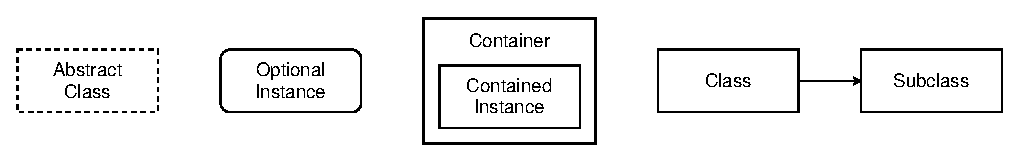
\includegraphics{h_key.eps}
\end{figure}

\subsubsection{Line Structure}
\begin{figure}[ht]
\centering
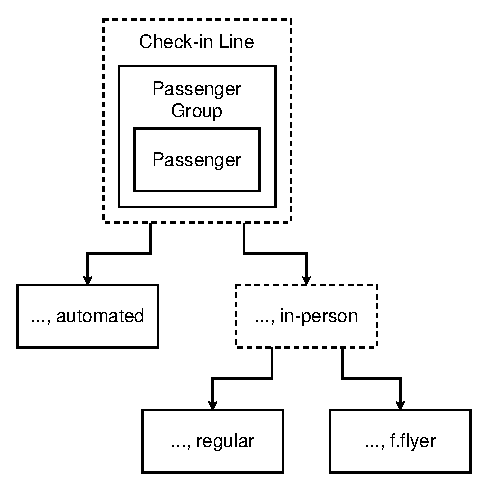
\includegraphics{h_line.eps}
\end{figure}

\pagebreak

\subsubsection{Counter Structure}
\begin{figure}[ht]
\centering
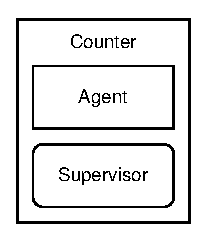
\includegraphics{h_counter.eps}
\end{figure}

\subsection{Operation Sequence}
\begin{figure}[ht]
\centering
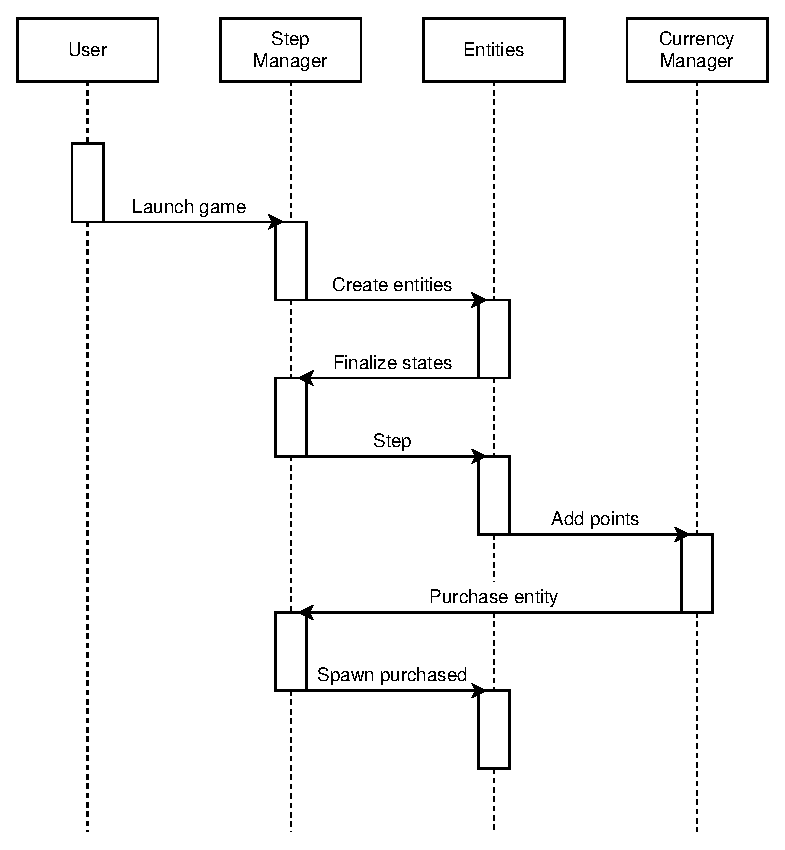
\includegraphics[scale=0.97]{s_operation.eps}
\end{figure}

\section{Signatures}

\pagebreak

\subsection{Passenger}
\begin{verbatim}
    class Passenger {
        
        private boolean frequent;
        private boolean excessBaggage;
        private boolean complexRoute;
        private boolean overbooked;
        ...
        protected Passenger() { ... }
        ...
    }
\end{verbatim}

\subsection{Passenger Group}
\begin{verbatim}
    class PassengerGroup {
        
        private List passengers;
        ...
        protected PassengerGroup() { ... }
        ...
    }
\end{verbatim}

\subsection{Check-in Line}
\begin{verbatim}
    abstract class Line {
        
        private List passengerGroups;
        ...
    }
\end{verbatim}

\subsection{Check-in Line, automated}
\begin{verbatim}
    class AutomatedLine extends Line {
        
        protected AutomatedLine(Counter c) { ... }

        // sends the front PassengerGroup to the next open counter section,
        // if available
        private void sendToCounter() { ... }
        ...
    }
\end{verbatim}

\subsection{Check-in Line, in-person}
\begin{verbatim}
    abstract class PersonalLine extends Line {
        
        // wait for the next group to be called to the counter
        private void waitForCall() { ... }
        ...
    }
\end{verbatim}

\pagebreak

\subsection{Check-in Line, regular}
\begin{verbatim}
    class RegularLine extends PersonalLine {
        
        protected RegularLine(Counter c) { ... }
        ...
    }
\end{verbatim}

\subsection{Check-in Line, frequent-flyer}
\begin{verbatim}
    class FrequentLine extends PersonalLine {
        
        protected FrequentLine(Counter c) { ... }

        protected void queueGroup(PassengerGroup group) { ... }
        ...
    }
\end{verbatim}

\subsection{Counter}
\begin{verbatim}
    class Counter {

        private Agent[] stations;
        
        protected Counter(Line q) { ... }

        protected void addAgent(Agent a, int i) { ... }
        protected void addSupervisor(Supervisor a, i) { ... }
        ...
    }
\end{verbatim}

\subsection{Agent}
\begin{verbatim}
    class Agent {
        
        protected Agent() { ... }
        ...
    }
\end{verbatim}

\subsection{Supervisor}
\begin{verbatim}
    class Supervisor extends Agent {
        
        protected Supervisor() { super(); ... }
        ...
    }
\end{verbatim}

\subsection{Manager, Currency}
\begin{verbatim}
    public final class CurrencyManager {
        
        private static final CurrencyManager cm_instance =
            new CurrencyManager();

        private CurrencyManager() { ... }
        ...
        public static CurrencyManager getInstance() {
            return cm_instance;
        }
        ...
    }
\end{verbatim}

\subsection{Manager, Step}
\begin{verbatim}
    public final class StepManager {
        
        private static final StepManager sm_instance =
            new StepManager();
            
        private StepManager() { ... }
        ...
        public static StepManager getInstance() {
            return sm_instance;
        }
        ...
    }
\end{verbatim}

\end{document}
